
    \subsection*{Параметры: $T=2$, $\Delta t=0.01$, $V=12$, $\Delta \nu=0.01$}

    \begin{figure}[H]
        \centering
        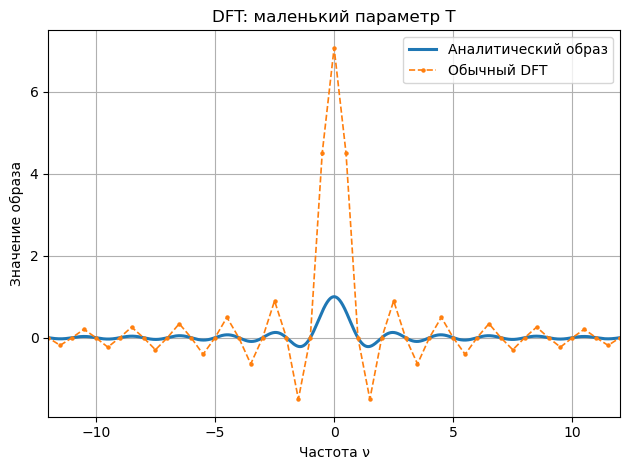
\includegraphics[width=0.8\textwidth]{task1/figs_1_5/dft_bad_T_spectrum.png}
        \caption{Спектр сигнала $\Pi(t)$ (численный FFT и аналитический sinc)}
    \end{figure}
Функция имеет много "острых" углов, требуется более точное приближение.

    
\subsection*{Параметры: $T=10$, $\Delta t=0.01$, $V=12$, $\Delta \nu=0.01$}

    \begin{figure}[H]
        \centering
        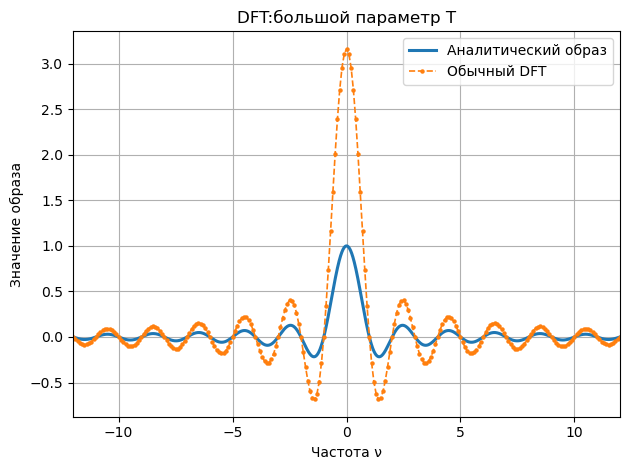
\includegraphics[width=0.8\textwidth]{task1/figs_1_5/dft_good_T_spectrum.png}
        \caption{Спектр сигнала $\Pi(t)$ (численный FFT и аналитический sinc)}
    \end{figure}
Функция стала более гладкой, спектр стал ближе к аналитическому sinc-образному виду.


    \subsection*{Параметры: $T=10$, $\Delta t=0.1$, $V=10$, $\Delta \nu=0.01$}
    \begin{figure}[H]
        \centering
        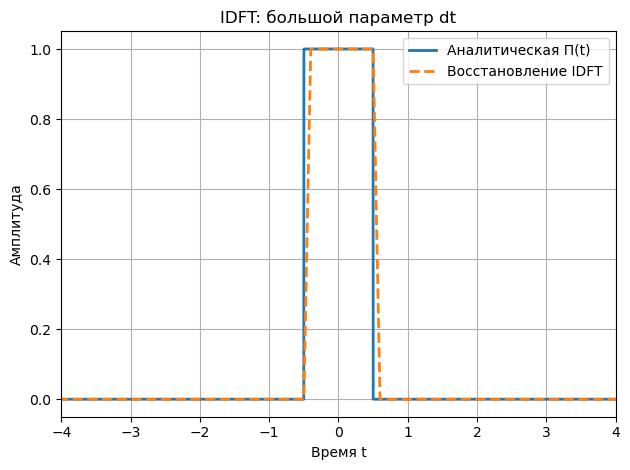
\includegraphics[width=0.8\textwidth]{task1/figs_1_5/dft_bad_dt_reconstruction.png}
        \caption{Восстановление сигнала $\Pi(t)$ методом FFT}
    \end{figure}
    
    \subsection*{Параметры: $T=10$, $\Delta t=0.001$, $V=10$, $\Delta \nu=0.01$}

    \begin{figure}[H]
        \centering
        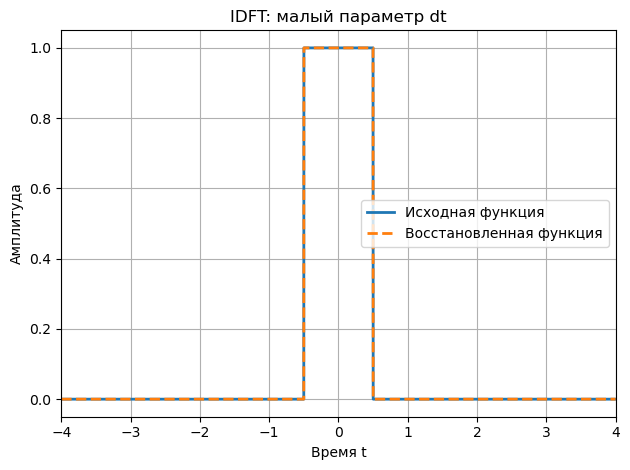
\includegraphics[width=0.8\textwidth]{task1/figs_1_5/dft_good_dt_reconstruction.png}
        \caption{Восстановление сигнала $\Pi(t)$ методом FFT}
    \end{figure}
Точность приближения восстановленной функции значительно улучшилась.